\section{Task 3}

\subsection{a)}

\begin{figure}[H]
\centering
\begin{circuitikz}[american voltages]

    % Bridge nodes
    \node[circle, fill=black, inner sep=0pt] (Top) at (0,2) {};
    \node[circle, fill=black, inner sep=0pt] (Right) at (2,0) {};
    \node[circle, fill=black, inner sep=0pt] (Bottom) at (0,-2) {};
    \node[circle, fill=black, inner sep=0pt] (Left) at (-2,0) {};

    % Source (input) inside bridge
    \draw (Top) to[open, v^=$U_i$] (Bottom);

    % Diodes (bridge)
    \draw (Top) to[D, l=$D_1$] (Right);
    \draw (Right) to[D, l=$D_2$] (Bottom);
    \draw (Bottom) to[D, l=$D_3$] (Left);
    \draw (Left) to[D, l=$D_4$] (Top);

    % Output resistor
    \node[circle, fill=black, inner sep=0pt] (OutTop1) at (4,0) {};
    \node[circle, fill=black, inner sep=0pt] (OutBot1) at (4,-3) {};
    \node[circle, fill=black, inner sep=0pt] (OutBot2) at (-2,-3) {};

    \draw (Right) -- (OutTop1);
    \draw (Left) -- (OutBot2);
    \draw (OutBot1) -- (OutBot2);

    \draw (OutTop1) to[R=$R$] (OutBot1);

    % Output voltage
    \draw (5, 0) to[open, l^=$U_0$] (5, -3);

    \node[ground] at (OutBot1) {};

    \draw[->, thick] (Top) -- (Right);
    \draw[->, thick] (Right) -- (OutTop1);
    \draw[->, thick] (OutBot1) -- (OutBot2);
    \draw[->, thick] (Left) -- (Bottom);
    \draw[->, thick] (Bottom) -- (Top);

\end{circuitikz}
\caption{Current direction in positive cycle}
\label{fig:bridge_rectifier}
\end{figure}

\begin{figure}[H]
\centering
\begin{circuitikz}[american voltages]

    % Bridge nodes
    \node[circle, fill=black, inner sep=0pt] (Top) at (0,2) {};
    \node[circle, fill=black, inner sep=0pt] (Right) at (2,0) {};
    \node[circle, fill=black, inner sep=0pt] (Bottom) at (0,-2) {};
    \node[circle, fill=black, inner sep=0pt] (Left) at (-2,0) {};

    % Source (input) inside bridge
    \draw (Top) to[open, v^=$U_i$] (Bottom);

    % Diodes (bridge)
    \draw (Top) to[D, l=$D_1$] (Right);
    \draw (Right) to[D, l=$D_2$] (Bottom);
    \draw (Bottom) to[D, l=$D_3$] (Left);
    \draw (Left) to[D, l=$D_4$] (Top);

    % Output resistor
    \node[circle, fill=black, inner sep=0pt] (OutTop1) at (4,0) {};
    \node[circle, fill=black, inner sep=0pt] (OutBot1) at (4,-3) {};
    \node[circle, fill=black, inner sep=0pt] (OutBot2) at (-2,-3) {};

    \draw (Right) -- (OutTop1);
    \draw (Left) -- (OutBot2);
    \draw (OutBot1) -- (OutBot2);

    \draw (OutTop1) to[R=$R$] (OutBot1);

    % Output voltage
    \draw (5, 0) to[open, l^=$U_0$] (5, -3);

    \node[ground] at (OutBot1) {};

    \draw[->, thick] (Bottom) -- (Right);
    \draw[->, thick] (Right) -- (OutTop1);
    \draw[->, thick] (OutBot1) -- (OutBot2);
    \draw[->, thick] (Left) -- (Top);
    \draw[->, thick] (Top) -- (Bottom);

\end{circuitikz}
\caption{Current direction in negative cycle}
\label{fig:bridge_rectifier}
\end{figure}


\noindent
Current in both cases flow in the same direction through the resistor, $R$. The diodes are ideal and there is no voltage drop over any component, except for the resistor. So the fall of potential over the resistor must equal the total input voltage. We can graph it as shown below.

\begin{figure}[H]
\centering
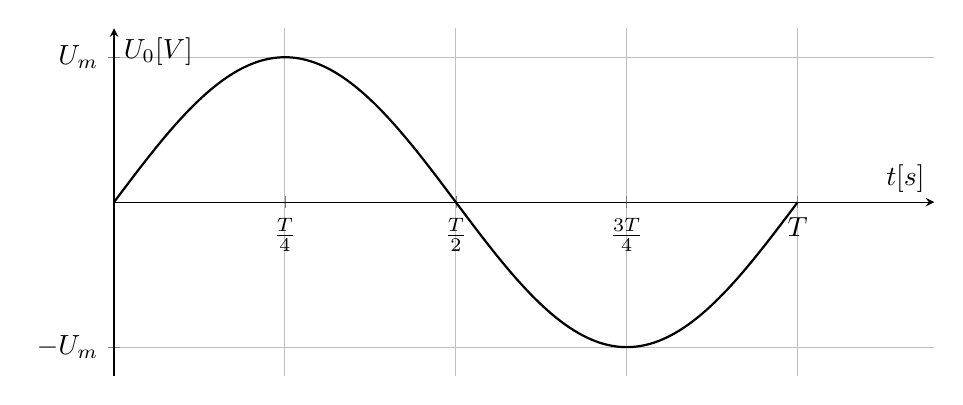
\begin{tikzpicture}
\begin{axis}[
    width=12cm,
    height=6cm,
    xlabel={$t [s]$},
    ylabel={$U_0 [V]$},
    xmin=0, xmax=1.2,
    ymin=-1.2, ymax=1.2,
    axis lines=middle,
    xtick={0,0.25,0.5,0.75,1},
    xticklabels={$0$, $\frac{T}{4}$, $\frac{T}{2}$, $\frac{3T}{4}$, $T$},
    ytick={-1,1},
    yticklabels={$-U_m$, $U_m$},
    grid=both,
    domain=0:1,
    samples=200
]

\addplot[thick]
{sin(deg(2*pi*x))};

\end{axis}
\end{tikzpicture}
\caption{Voltage over resistor.}
\end{figure}

\subsection{b)}

\begin{figure}[H]
\centering
\begin{circuitikz}[american voltages]

    % Bridge nodes
    \node[circle, fill=black, inner sep=0pt] (Top) at (0,2) {};
    \node[circle, fill=black, inner sep=0pt] (Right) at (2,0) {};
    \node[circle, fill=black, inner sep=0pt] (Bottom) at (0,-2) {};
    \node[circle, fill=black, inner sep=0pt] (Left) at (-2,0) {};

    % Source (input) inside bridge
    \draw (Top) to[open, v^=$U_i$] (Bottom);

    % Diodes (bridge)
    \draw (Top) to[D, l=$D_1$] (Left);
    \draw (Bottom) to[D, l=$D_3$] (Left);
    \draw (Right) to[D, l=$D_2$] (Top);
    \draw (Right) to[D, l=$D_4$] (Bottom);

    % Output resistor
    \node[circle, fill=black, inner sep=0pt] (OutTop1) at (4,0) {};
    \node[circle, fill=black, inner sep=0pt] (OutBot1) at (4,-3) {};
    \node[circle, fill=black, inner sep=0pt] (OutBot2) at (-2,-3) {};

    \draw (Right) -- (OutTop1);
    \draw (Left) -- (OutBot2);
    \draw (OutBot1) -- (OutBot2);

    \draw (OutTop1) to[R=$R$] (OutBot1);

    % Output voltage
    \draw (5, 0) to[open, l^=$U_0$] (5, -3);

    \node[ground] at (OutBot1) {};

    \draw[->, thick] (Top) -- (Left);
    \draw[->, thick] (OutTop1) -- (Right);
    \draw[->, thick] (OutBot2) -- (OutBot1);
    \draw[->, thick] (Right) -- (Bottom);
    \draw[->, thick] (Bottom) -- (Top);

\end{circuitikz}
\caption{Current direction in positive cycle}
\label{fig:bridge_rectifier}
\end{figure}


\begin{figure}[H]
\centering
\begin{circuitikz}[american voltages]

    % Bridge nodes
    \node[circle, fill=black, inner sep=0pt] (Top) at (0,2) {};
    \node[circle, fill=black, inner sep=0pt] (Right) at (2,0) {};
    \node[circle, fill=black, inner sep=0pt] (Bottom) at (0,-2) {};
    \node[circle, fill=black, inner sep=0pt] (Left) at (-2,0) {};

    % Source (input) inside bridge
    \draw (Top) to[open, v^=$U_i$] (Bottom);

    % Diodes (bridge)
    \draw (Top) to[D, l=$D_1$] (Left);
    \draw (Bottom) to[D, l=$D_3$] (Left);
    \draw (Right) to[D, l=$D_2$] (Top);
    \draw (Right) to[D, l=$D_4$] (Bottom);

    % Output resistor
    \node[circle, fill=black, inner sep=0pt] (OutTop1) at (4,0) {};
    \node[circle, fill=black, inner sep=0pt] (OutBot1) at (4,-3) {};
    \node[circle, fill=black, inner sep=0pt] (OutBot2) at (-2,-3) {};

    \draw (Right) -- (OutTop1);
    \draw (Left) -- (OutBot2);
    \draw (OutBot1) -- (OutBot2);

    \draw (OutTop1) to[R=$R$] (OutBot1);

    % Output voltage
    \draw (5, 0) to[open, l^=$U_0$] (5, -3);

    \node[ground] at (OutBot1) {};

    \draw[->, thick] (Bottom) -- (Left);
    \draw[->, thick] (OutTop1) -- (Right);
    \draw[->, thick] (OutBot2) -- (OutBot1);
    \draw[->, thick] (Right) -- (Top);
    \draw[->, thick] (Top) -- (Bottom);

\end{circuitikz}
\caption{Current direction in negative cycle}
\label{fig:bridge_rectifier}
\end{figure}

\noindent
The only drop of voltage is over the resistor, but now the current is reversed. So the graph is the negative of the input.

\begin{figure}[H]
\centering
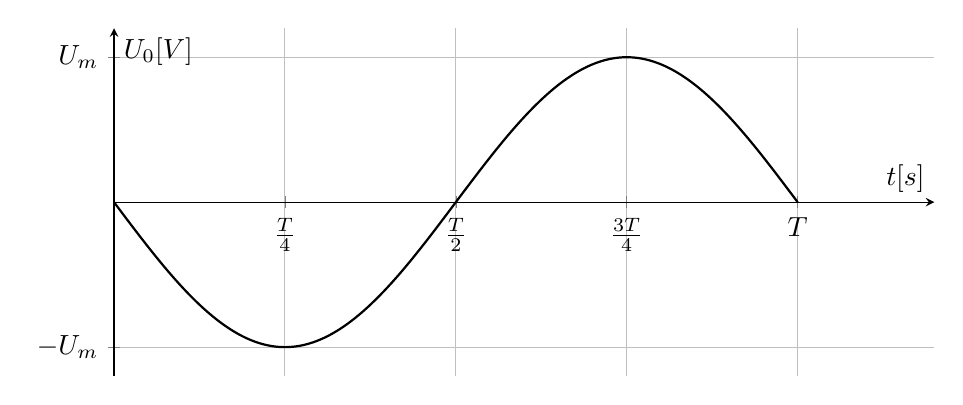
\begin{tikzpicture}
\begin{axis}[
    width=12cm,
    height=6cm,
    xlabel={$t [s]$},
    ylabel={$U_0 [V]$},
    xmin=0, xmax=1.2,
    ymin=-1.2, ymax=1.2,
    axis lines=middle,
    xtick={0,0.25,0.5,0.75,1},
    xticklabels={$0$, $\frac{T}{4}$, $\frac{T}{2}$, $\frac{3T}{4}$, $T$},
    ytick={-1,1},
    yticklabels={$-U_m$, $U_m$},
    grid=both,
    domain=0:1,
    samples=200
]

\addplot[thick]
{-sin(deg(2*pi*x))};

\end{axis}
\end{tikzpicture}
\caption{Voltage over resistor.}
\end{figure}